\section{InceptionTime Network}
Po przeanalizowaniu architektury ResNet18, przyjrzymy się teraz
sieci InceptionTime, która jest architekturą specjalnie zaprojektowaną
do pracy z przebiegami czasowymi. Architektura ta została zaproponowana
w pracy \cite{ismail2020inceptiontime} i opiera się w głównej mierze na
trzech warstwach konwolucyjnych, o różnej długości jądra konwolucyjnego,
które są połączone równolegle. Pozwala to na wychwycenie zarówno lokalnych,
jak i globalnych zależności w danych wejściowych. Możemy rozpatrywać architekturę
InceptionTime Network na trzech poziomach szczegółowości. Na najwyższym poziomie, sieć
składa się z dwóch bloków połączonych szeregowo. Każdy z tych bloków składa się z trzech
warstw InceptionModule, które są połączone znowu szeregowo. Natomiast najciekawsze jest to,
co dzieje się na najniższym poziomie, czyli w samym module InceptionModule.
\begin{figure}[H]
  \centering
  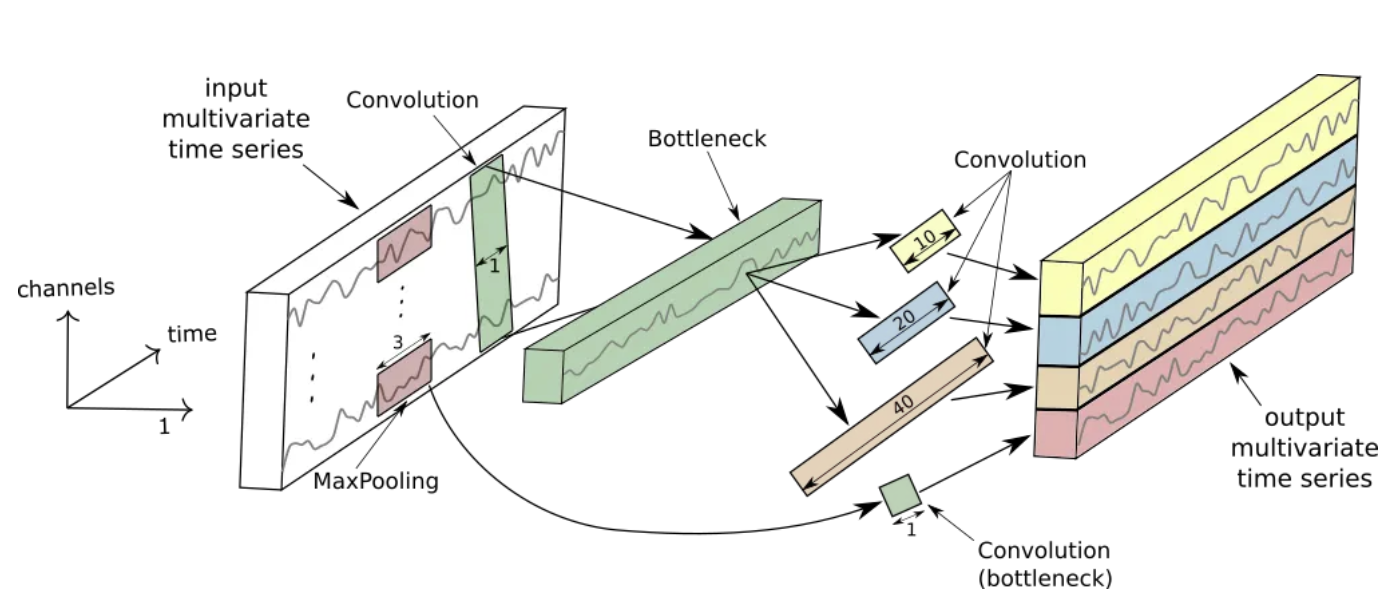
\includegraphics[width=0.8\textwidth]{Inception_time/image.png}
  \caption{Budowa InceptionModule. \cite{ismail2020inceptiontime}}
  \label{fig:inception_module}
\end{figure}
Jak widać na Rysunku \ref{fig:inception_module}, centralną częścią tego modułu są trzy warstwy
konwolucyjne o różnych rozmiarach jądra konwolucyjnego (w pracy są to odpowiednio 10, 20 i 40,
  natomiast w naszej implementacji są to odpowiednio 9, 19 i 39, tak aby nie pojawiały się problemy
z paddingiem). Zauważmy również, że podobnie jak w ResNet, mamy tutaj połączenie rezydualne, z podobnego
powodu, czyli aby zapobiec problemowi znikającego gradientu. Oprócz tego, należy zauważyć obecność dwóch
warstw bottleneck, które służą do dopasowania liczby kanałów wejściowych i wyjściowych. Należy zauważyć, że
architekura tej sieci czerpie z pomysłów znanych z ResNet, ale je znacząco rozwija w obrębie pojednynczego bloku.